% Short version only: what LayerTree costs against a bare UTXO, Lightning,
% Ark and transaction trees, condensed from design/cost-comparison.md
% for the developer reader. Every number is spec 0.12.1's (sections 4.5
% and 11, spec/scripts/sizes.md, spec/scripts/weights.md,
% spec/fee-analysis.md). The figures are the PDF twins of
% design/figures/*.svg, written by tools/gen_cost_figures.py --pdf-dir
% paper/figures. Tables both versions carry are table-*.tex; the full
% version prints them in its cost section and Appendix C instead.
\section{Costs Against the Alternatives}\label{app:compare}

Joining, updating and leaving a shared output each cost more bytes than
the same operation on a bare UTXO. What the sharing buys is a different
placement of the cost. Entry is close to free in bulk, value moves
off-chain for nothing, a bulk exit costs about a bare spend, and a solo
exit costs about nine times one but is a single transaction with no
timelock and no counterparty. This appendix walks through each of those
claims with the measured figures, then says where LayerTree loses and how
the numbers are made (\S\ref{app:cmp-model}).

\subsection{The Unit of Cost}\label{app:cmp-unit}

Every LayerTree operation is one transaction that spends the tree output
and recreates it. The witness carries a leaf and its Merkle path, and the
script folds the path twice, once to check the old root and once to
compute the new one. Each level costs 88 bytes of script and 41 of
witness in FULL, 129 weight units or about $32\vB$. The depth $D$ is fixed
when the tree is created, so an exit from a given tree is a constant size
whatever the population: $1{,}020\vB$ at $D = 16$, which holds 65{,}536
slots.

\begin{figure}[htbp]
\centering
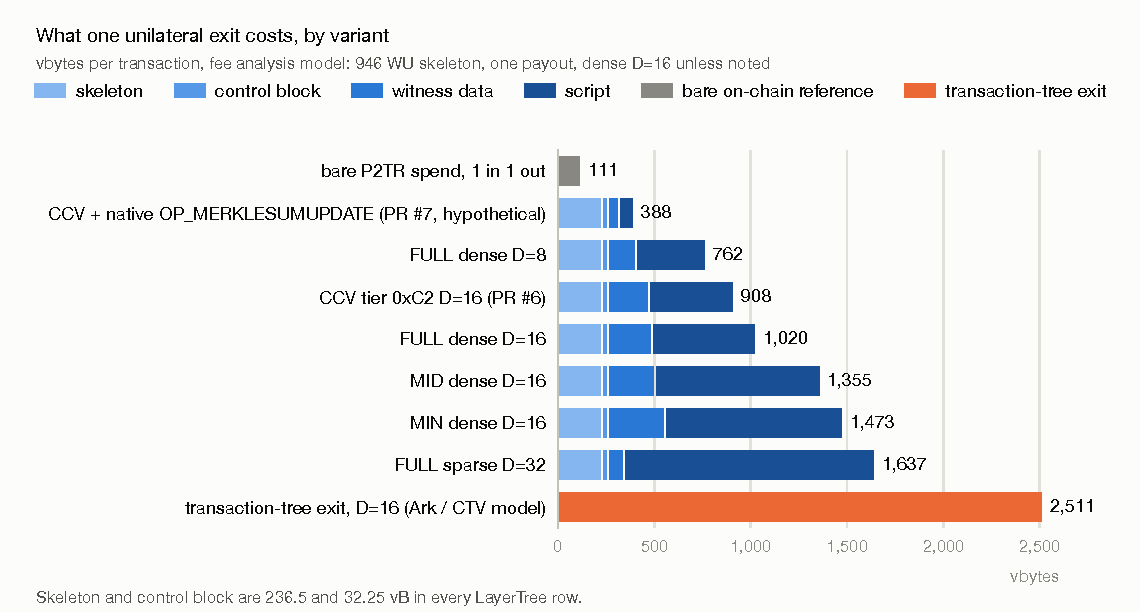
\includegraphics[width=\linewidth]{figures/exit-anatomy.pdf}
\caption{One unilateral exit by variant. The skeleton ($236.5\vB$) and
control block ($32.25\vB$) are the same in every LayerTree row; the
script dominates because tapscript has no loops and the levels are
unrolled. The sparse and native-opcode rows are measured on the
simulator's six-leaf tree. The ``PR'' labels name the repository
changes that added the CCV tier and the hypothetical opcode.}
\label{fig:cmp-anatomy}
\end{figure}

Figure~\ref{fig:cmp-anatomy} splits the exit into its parts, and
Table~\ref{tab:cmp-exit} lists every variant against a bare spend. MID
and MIN pay more for the same work because they lack the restored
arithmetic and point opcodes; CCV saves about a tenth by letting
\op{CHECKCONTRACTVERIFY} bind the state. The hypothetical native
Merkle-sum opcode of spec~13 item~12 is a measurement, never a tier: on
the simulator's six-leaf tree its exit is $388\vB$, with 252 bytes of
script at any depth, but the witness still carries one 40-byte sibling
per occupied level, so a full depth-16 tree costs about $520\vB$. That is
the floor for any design that publishes a proof and checks it in script.
The transaction-tree row is the model of \S\ref{sec:eval}: $D$
transactions of about $150\vB$ to unroll the branch, plus a $111\vB$
claim. It flatters the tree, since it omits the relative timelock at the
leaf and the fee each of the 16 transactions pays separately;
Table~\ref{tab:ark} gives the same model at other round sizes and radix~4.

\begin{table}[htbp]
\centering
\caption{One exit, dense $D = 16$ unless noted. Model: the transaction model of \S\ref{app:cmp-model}. Serialised: the real transaction the test suites build, with the witness length prefixes the model leaves out (\texttt{spec/scripts/weights.md}).}
\label{tab:cmp-exit}
\setlength{\tabcolsep}{4pt}\scriptsize
\begin{tabular}{@{}lrr@{}}
\toprule
variant & model (vB) & serialised (vB) \\
\midrule
bare P2TR spend, one input and one output & 111 & \\
one P2TR output inside a batch transaction & 43 & \\
FULL \tr{EXIT}$_1$ & 1{,}020 & 1{,}030 \\
FULL, fee taken from the payout & 921 & \\
FULL, $D = 8$ and $D = 20$ & 762 and 1{,}149 & \\
FULL tower exit \tr{EXIT}$_1^{t}$ & 1{,}046 & \\
FULL sparse $D = 32$, six-leaf tree & 1{,}637 & 1{,}648 \\
FULL sparse $D = 32$, $2^{16}$ members (measured) & \sparseExitBig & \\
MID & 1{,}355 & 1{,}398 \\
MIN & 1{,}473 & 1{,}518 \\
CCV, tapleaf \texttt{0xC2} & 908 & 918 \\
native Merkle-sum opcode (hypothetical), six-leaf tree & 388 & \\
native Merkle-sum opcode (hypothetical), full $D = 16$ tree & $\approx 520$ & \\
radix-2 transaction-tree exit (model) & 2{,}511 & \\
\bottomrule
\end{tabular}
\end{table}

% The transaction-tree model across round sizes, shared by both versions:
% Appendix C of the full version (appendix-eval.tex) and the short
% version's cost appendix (appendix-compare.tex).

\begin{table}[tbp]
\centering
\caption{The transaction-tree model across round sizes $N$. A level is one key-path P2TR input and $r$ P2TR outputs, $68 + 43r\vB$ (154 at radix 2, used as 150; 240 at radix 4); the claim is a plain P2TR spend, $111\vB$; anchors and their fee children are omitted, which favours the tree. Mass exit: the tree's interior shared by all members, against LayerTree's \tr{REWRITE}$_6$ or sweep of a 64-slot cohort. LayerTree is measured at $D = \log_2 N$.}
\label{tab:ark}
\setlength{\tabcolsep}{5pt}\scriptsize
\begin{tabular}{@{}lrrr@{}}
\toprule
 & LayerTree, dense & radix-2 tree & radix-4 tree \\
\midrule
isolated exit, $N = 2^{8}$ & 762 & 1{,}311 & 1{,}071 \\
isolated exit, $N = 2^{12}$ & 891 & 1{,}911 & 1{,}551 \\
isolated exit, $N = 2^{16}$ & 1{,}020 & 2{,}511 & 2{,}031 \\
mass exit, per member & 158 to 162 & $\approx 261$ & $\approx 191$ \\
\bottomrule
\end{tabular}
\end{table}


\subsection{Exits in Bulk}\label{app:cmp-bulk}

A single exit is the expensive case. The cost per leaf falls as more
leaves leave in one transaction, and how far it falls depends on who has
to sign (Figure~\ref{fig:cmp-amortise}, Table~\ref{tab:batch}).

\emph{Owners who coordinate} leave together with \tr{EXIT}$_K$. Each leaf
still carries its own path, so \tr{EXIT}$_2$ is $1{,}684\vB$: $842\vB$ a
leaf, and $665\vB$ for the second exit alone. \emph{The operator} sweeps
an aligned cohort of expired leases with \tr{EVICT\_SUBTREE}$_h$, which
publishes the cohort's leaves once and shares the path above it: $203\vB$
a leaf for 13 leaves at $h = 4$, $158\vB$ for 51 at $h = 6$, and about
$147\vB$ for the 205 leaves of a height-8 cohort at $D = 20$. The sweep
needs no member, but it only works on leaves whose evictor is the
operator and whose lease has run out. A leaf with the \NUMS{} evictor, or
with a lease far in the future, blocks the sweep of its whole cohort
(spec~7.7), so the operator's cheap removal is something members opt
into at join time by accepting a lease.

\emph{Owners who want the sweep's price without a lease} use the cohort
rewrite \tr{REWRITE}$_h$ (\S\ref{sec:ops}) with every position leaving.
It is the same post-order fold, authorised by one plain signature per
leaf and the operator's, with no nonce round. At $D = 16$ four owners
leaving a height-2 cohort pay $366\vB$ each, sixteen at $h = 4$ pay
$202\vB$, and sixty-four at $h = 6$ pay $165\vB$, within seven vbytes of
the operator's sweep. The same script settles a cohort in place:
rotating every key of a height-6 cohort is $151\vB$ per changed leaf
against $1{,}030\vB$ for an \tr{UPDATE} each, and a position that does
not change costs about $95\vB$ and needs no signature, so an absent
member is carried through rather than excluded.

\begin{figure}[htbp]
\centering
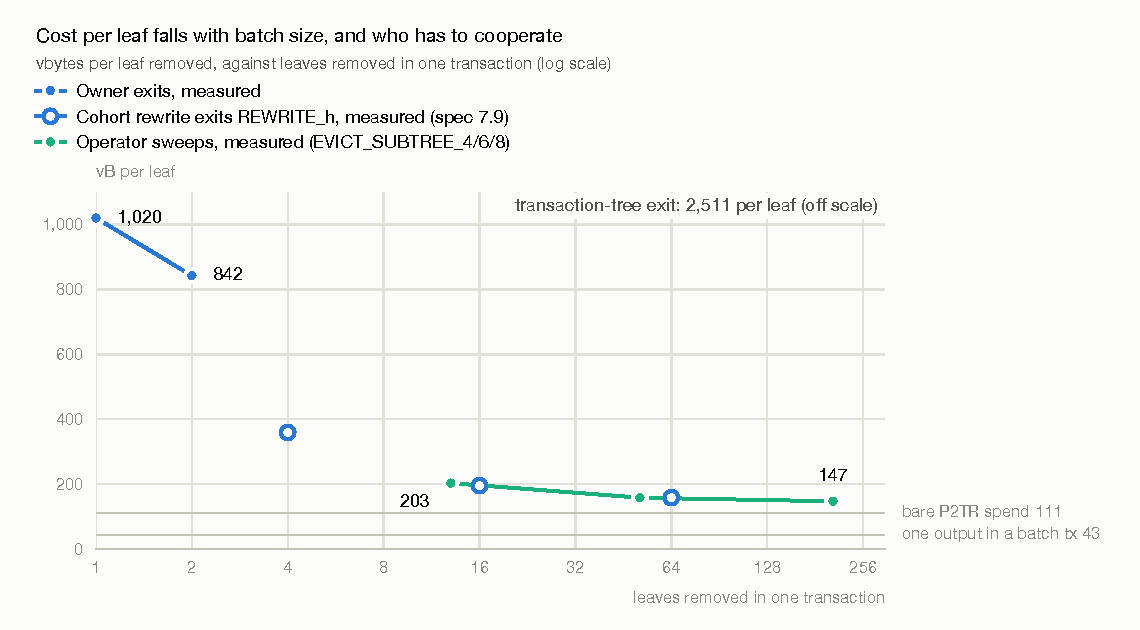
\includegraphics[width=\linewidth]{figures/exit-amortisation.pdf}
\caption{Cost per leaf against leaves removed in one transaction (log
scale): owner exits (\tr{EXIT}$_1$, \tr{EXIT}$_2$), owners leaving by
\tr{REWRITE}$_h$ ($366$, $202$ and $165\vB$ at 4, 16 and 64 positions),
and operator sweeps (\tr{EVICT\_SUBTREE}$_{4,6,8}$: 13, 51 and 205
leaves).}
\label{fig:cmp-amortise}
\end{figure}

\begin{figure}[htbp]
\centering
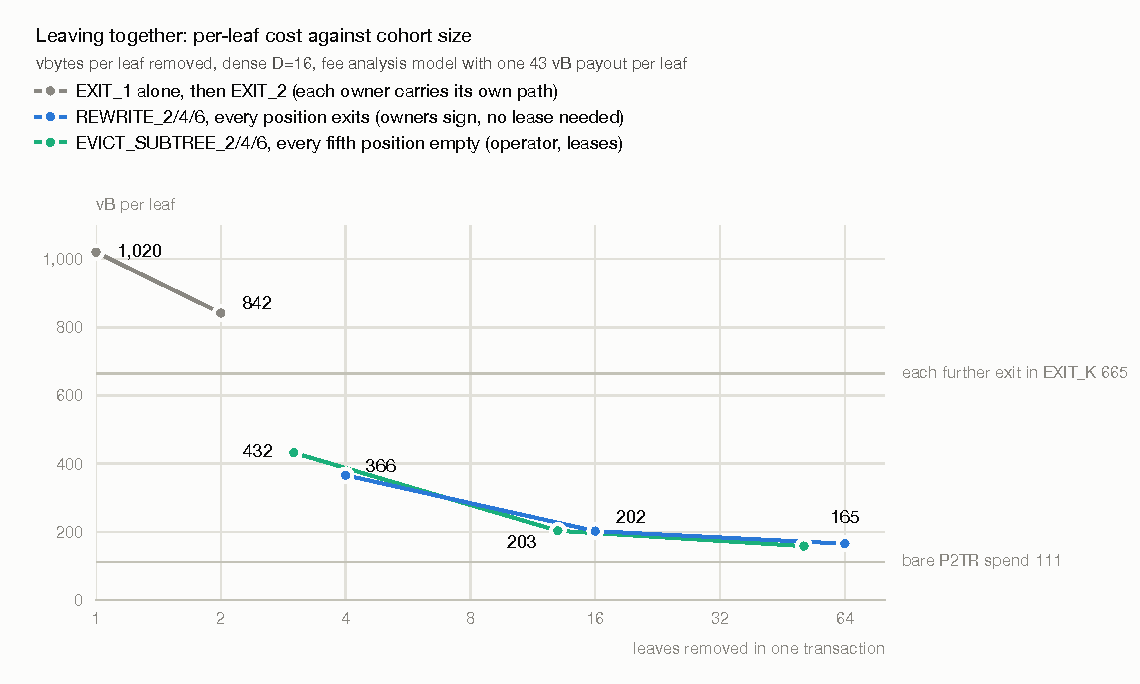
\includegraphics[width=\linewidth]{figures/cohort-cost.pdf}
\caption{The same three ways out at $D = 16$, per leaf removed against
the number removed in one transaction: owners alone or in pairs, owners
leaving together by \tr{REWRITE}$_h$, and the operator's sweep. The
rewrite starts below the \tr{EXIT}$_K$ floor and meets the sweep near
$h = 6$ ($165$ against $158\vB$ per leaf).}
\label{fig:cmp-cohort}
\end{figure}

% The batch-shape table, shared by both versions: the full version's
% evaluation section (body-eval.tex) and the short version's cost
% appendix (appendix-compare.tex).

\begin{table}[tbp]
\centering
\caption{Batch shapes at dense $D = 16$ on the transaction model: vB per leaf that leaves or changes, or per member that joins. Self-funded joins add each member's P2TR key-path funding input ($58\vB$) and the signing round of \S\ref{sec:parties}. The \tr{REWRITE}$_h$ rows are FULL's figures.}
\label{tab:batch}
\setlength{\tabcolsep}{4pt}\scriptsize
\begin{tabular}{@{}lrrr@{\quad}lrrr@{}}
\toprule
removal & leaves & tx & per leaf & addition or change & leaves & tx & per leaf \\
\midrule
\tr{EXIT}$_1$ & 1 & 1{,}020 & 1{,}020 & \tr{JOIN}$_0$ & 1 & 937 & 937 \\
\tr{EXIT}$_2$ & 2 & 1{,}684 & 842 & \tr{JOIN}$_2$ & 4 & 872 & 218 \\
\tr{EVICT\_SUBTREE}$_4$ & 13 & 2{,}638 & 203 & \tr{JOIN}$_8$ (operator-funded) & 256 & 679 & 2.7 \\
\tr{EVICT\_SUBTREE}$_6$ & 51 & 8{,}057 & 158 & sparse \tr{JOIN}$_0$, $D = 32$ & 1 & 1{,}601 & 1{,}601 \\
\tr{REWRITE}$_2$, all leave & 4 & 1{,}455 & 364 & \tr{REWRITE}$_6$, keys rotated & 64 & 9{,}496 & 148 \\
\tr{REWRITE}$_6$, all leave & 64 & 10{,}392 & 162 & \tr{UPDATE}, one leaf & 1 & 1{,}030 & 1{,}030 \\
\bottomrule
\end{tabular}
\end{table}


Batching changes what the chain limit counts. Every transition spends
the same output, so unconfirmed transitions form a chain, and relay
policy caps it: 25 transactions under the ancestor and descendant limits
of Bitcoin Core before 31.0~\cite{corepolicy}, at most 64 under cluster
mempool~\cite{clustermempool} ($\kappa$ of \S\ref{sec:liveness}). The cap
counts transactions, not leaves, so a 51-leaf sweep is one entry.
Uncoordinated exits chain only if each exiter rebuilds on the previous
unconfirmed exit, or a tower or the operator holding \tr{EXIT}$^{t}$
authorisations builds them in sequence; otherwise they conflict and
replace one another. So 25 a block is the cooperative ceiling for single
exits, and the worst case is set by $\beta$. A deployment that expects
more shards into several trees, each sized by exit throughput rather
than by depth. Each batch shape is its own
tapleaf, and each doubling of the taptree adds $8\vB$ to every spend,
so a tree that carries the sweeps and rewrites (16 to 32 tapleaves) pays
8 to $16\vB$ more on every exit.

\subsection{Entry}\label{app:cmp-entry}

\tr{JOIN}$_h$ grafts a prebuilt subtree of height $h$ into an empty slot
and walks only the $D - h$ levels above it, so a bigger cohort is a
cheaper transaction (Figure~\ref{fig:cmp-join}). At $D = 16$ with no
payout output, as spec~11 prices a join, one member costs $937\vB$, a
four-member graft $872\vB$ ($218\vB$ a member), a 256-member graft
about $679\vB$ ($2.7\vB$) and a 1{,}024-member graft about $614\vB$
($0.6\vB$), both estimates from measured joins that walk as many levels, against $43\vB$ for one output in an on-chain batch
and about $154\vB$ for a channel opened in its own transaction.

\begin{figure}[htbp]
\centering
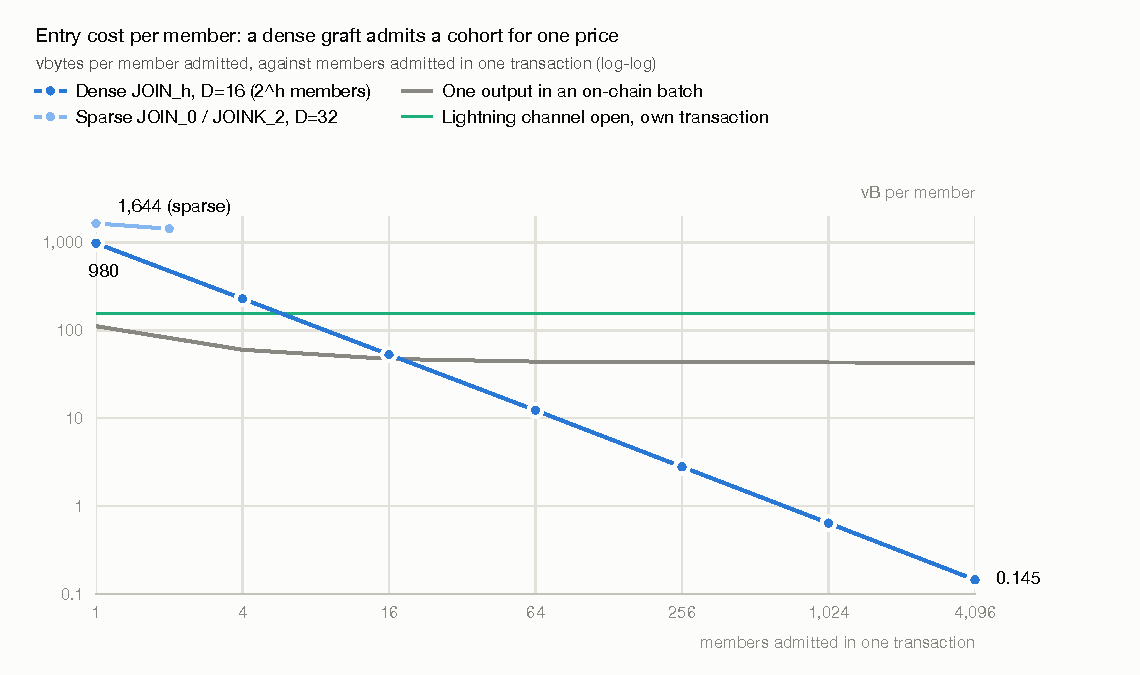
\includegraphics[width=\linewidth]{figures/join-amortisation.pdf}
\caption{Entry cost per member against members admitted in one
transaction (log-log). The figure prices each join with one payout
output, $43\vB$ above the no-payout pricing of spec~11 that the text and
Table~\ref{tab:batch} use: its 980 and 1{,}644 are 937 and 1{,}601 there.
The dense points above 4 members are extrapolated from the measured
\tr{JOIN}$_2$ at 129 weight units a level.}
\label{fig:cmp-join}
\end{figure}

Who funds the value grafted in decides who has to be online. When the
operator funds it from the transaction's fee input, the graft needs the
operator's signature alone, and the whole cohort costs nothing beyond
the figure; members pay for their balances off-chain after the graft
confirms, or beforehand with a hash-locked voucher (\S\ref{sec:vouchers}).
When each member funds its own leaf, each adds a key-path input of about
$58\vB$, the saving against an on-chain batch shrinks to the output side,
and the cohort becomes a signing round among the funders: every signature
commits to the new root, so a joiner who drops out invalidates the others
and the operator collects again (\S\ref{sec:parties}). Either way, a
member checks its own path inside the subtree before funding, because a
grafted node with no real tree behind it freezes its value. The sparse
profile cannot graft at all: a sparse join is one leaf for $1{,}601\vB$.

\subsection{Moving Value}\label{app:cmp-move}

On-chain transitions are the wrong path for payments. An \tr{UPDATE} at
$D = 16$ is $1{,}030\vB$ and a voucher redemption with \tr{CLAIM}
$1{,}618\vB$, priced as spec~11 prices them, without a payout output
($1{,}073$ and $1{,}661\vB$ on the skeleton that carries one), against
$111\vB$ for a bare spend. A member who moved value by rewriting its leaf
would pay about nine times what separate UTXOs pay per payment
(Table~\ref{tab:cmp-move}).

Value moves off-chain instead, and the chain carries only membership
changes and the exercise of exit rights. Payments between channel leaves
are ordinary HTLC forwards; their funding outputs do not exist until a
leaf exits (\S\ref{sec:channels}). A voucher is one signed message from
payer to payee, credit until redeemed, and an issuer usually settles it
off-chain rather than the holder redeeming it (\S\ref{sec:vouchers}).
\tr{UPDATE} is maintenance: resizing a balance, renewing a lease,
rotating a key. When a cohort's balances do have to settle on-chain,
\tr{REWRITE}$_h$ does it for about $151\vB$ per changed leaf with only the
changed leaves' owners signing, which is the settlement an Ark round
performs without the round.

\begin{table}[htbp]
\centering
\caption{1{,}000 members who each make 1{,}000 payments, entry and exit included where a design has them. The Lightning row opens and closes each channel cooperatively in its own transaction; the Ark row boards and leaves as outputs of round transactions, whose shared overhead is left out; the LayerTree rows enter by one 1{,}024-slot graft.}
\label{tab:cmp-move}
\setlength{\tabcolsep}{4pt}\scriptsize
\begin{tabular}{@{}lr@{}}
\toprule
how value moves & on-chain bytes \\
\midrule
bare UTXOs, one spend per payment & 111\,MvB \\
LayerTree, one on-chain \tr{UPDATE} per payment & 1{,}030\,MvB \\
Lightning channels, payments off-chain & 308\,kvB \\
Ark, payments off-chain (rounds and refreshes not priced) & 86\,kvB \\
LayerTree, payments off-chain, cohort exit or sweep (renewals not priced) & about 160\,kvB \\
LayerTree, payments off-chain, members never exit (balances sold by voucher) & under 1\,kvB \\
\bottomrule
\end{tabular}
\end{table}

\subsection{The Lightning Baseline and Lifetime per Member}\label{app:cmp-lifetime}

The Lightning figures are a simple taproot channel~\cite{taprootchans}
priced on the same model as the LayerTree rows, fee-bumping children
included (Table~\ref{tab:cmp-ln}). The non-taproot anchor commitment of
BOLT~3~\cite{bolt3} is $281\vB$ in place of the 240 used here.

\begin{table}[htbp]
\centering
\caption{A simple taproot channel on the transaction model.}
\label{tab:cmp-ln}
\setlength{\tabcolsep}{4pt}\scriptsize
\begin{tabular}{@{}lr@{}}
\toprule
transaction & vB \\
\midrule
funding: one P2TR key-path input, the funding output and change & 154 \\
cooperative close: the MuSig2 key-path spend of the funding output & 154 \\
commitment: a MuSig2 key-path input, two balance outputs and two anchors & 240 \\
anchor child that pays the commitment's fee & 152 \\
delayed sweep of the broadcaster's output after the CSV & 138 \\
force close: commitment, anchor child and sweep & 530 \\
\midrule
lifetime, open alone and force close & 684 \\
lifetime, open alone and cooperative close & 308 \\
lifetime, open as one output of a batch and cooperative close & 197 \\
lifetime, open as one output of a batch and force close & 573 \\
\bottomrule
\end{tabular}
\end{table}

Against this baseline a member who leaves a dense $D = 16$ tree alone
pays $1{,}020\vB$, about twice a channel's force close and 1.5 times its
684-byte lifetime. A channel leaf inside the tree costs its exit plus an
update, a settlement and their two anchor children, about $1{,}681\vB$ in
all, against $684\vB$ for a channel with its own funding output, because
materialising the funding output carries the Merkle-sum proof. The fair
comparison adds entry and exit for one member and asks how the member
leaves (Figure~\ref{fig:cmp-lifetime}, Table~\ref{tab:lifetime}).

\begin{figure}[htbp]
\centering
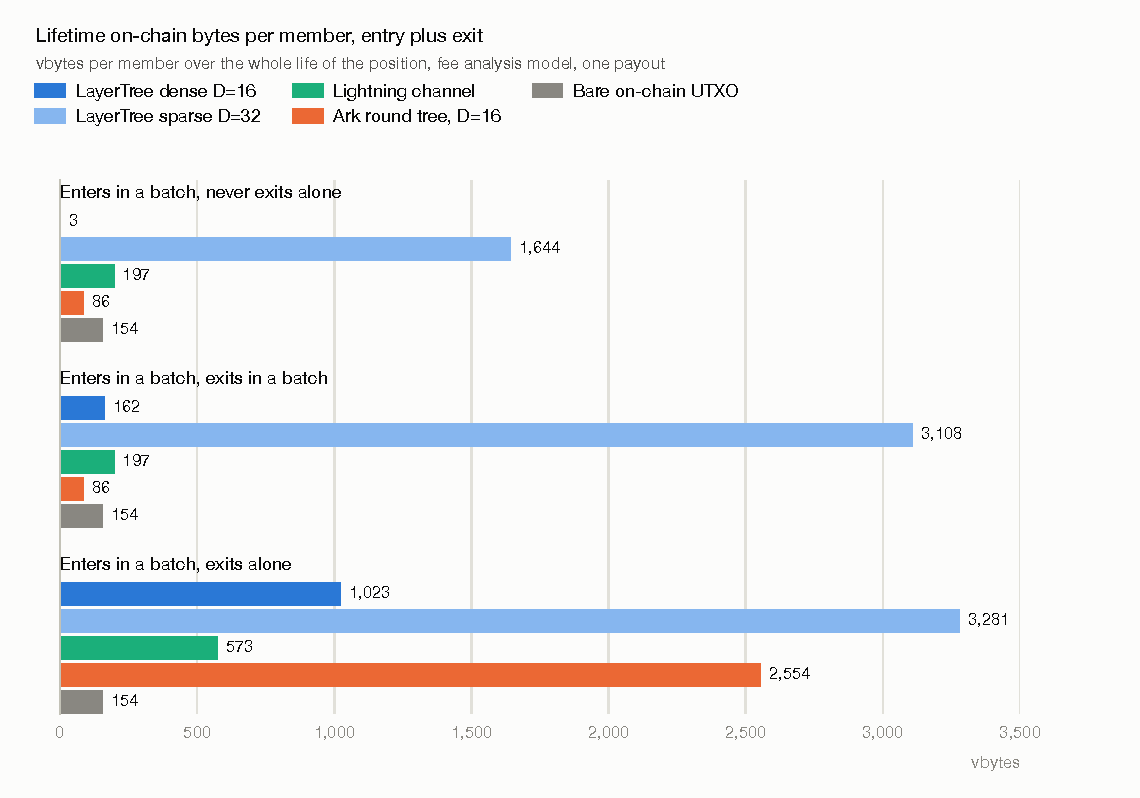
\includegraphics[width=\linewidth]{figures/lifetime.pdf}
\caption{Lifetime on-chain bytes per member, entry plus exit. The dense,
Lightning, Ark and bare rows are those of Table~\ref{tab:lifetime}. The
sparse bars price the join with a payout output and the exit on the
six-leaf tree (1{,}644, 3{,}108 and 3{,}281); Table~\ref{tab:sparse} gives the
sparse join and exit sizes, and the table above prices the join without a
payout output and the exit at $2^{16}$ members (1{,}601, 3{,}209 and
3{,}382).}
\label{fig:cmp-lifetime}
\end{figure}

% The lifetime table, shared by both versions: the full version's cost
% section (full-cost.tex) and the short version's cost appendix
% (appendix-compare.tex).

\begin{table}[tbp]
\centering
\caption{Lifetime on-chain bytes per member, by how it leaves, and the unilateral exit's latency (a tower watches for stale states; an Ark member must refresh before expiry). LayerTree rows are dense at $D = 16$ unless marked sparse. Entry is one $43\vB$ output in a shared transaction; for LayerTree it is a share of a 256-slot operator-funded graft, or that plus the member's $58\vB$ input when self-funded. LayerTree's batch exit is the 51-leaf sweep, which requires a lease. The sparse row enters by one sparse \tr{JOIN}$_0$ ($1{,}601\vB$, no payout output) and exits at the $2^{16}$-member estimate ($1{,}781\vB$), not the six-leaf measurement. Lightning is a simple taproot channel: cooperative close $154\vB$; force close a $240\vB$ commitment, its $152\vB$ anchor child and a $138\vB$ sweep. Ark's unilateral exit is the radix-2 unroll of its round.}
\label{tab:lifetime}
\setlength{\tabcolsep}{3pt}\scriptsize
\begin{tabular}{@{}lrrrlll@{}}
\toprule
 & \multicolumn{3}{c}{vB per member, leaving} & \multicolumn{3}{c}{unilateral exit} \\
\cmidrule(lr){2-4}\cmidrule(l){5-7}
 & never alone & in a batch & alone & txs & blocks & online \\
\midrule
LayerTree, operator-funded & 3 & 162 & 1{,}023 & 1 & 1 & nobody \\
LayerTree, self-funded & 61 & 220 & 1{,}081 & 1 & 1 & nobody \\
LayerTree sparse, $D = 32$ & 1{,}601 & 3{,}209 & 3{,}382 & 1 & 1 & nobody \\
Lightning channel & 197 & 197 & 573 & 3 & $\approx 145$ & tower \\
Ark, round of 256 & 86 & 86 & 1{,}354 & 9 & $8 +$ timelock & member \\
Ark, round of 65{,}536 & 86 & 86 & 2{,}554 & 17 & $16 +$ timelock & member \\
bare UTXO & 154 & 154 & 154 & 1 & 1 & nobody \\
\bottomrule
\end{tabular}
\end{table}


% Shared by both versions: the paragraph that reads the lifetime table
% (full-cost.tex, appendix-compare.tex).

\paragraph{Lifetime and latency.} Table~\ref{tab:lifetime} adds entry and
exit. The dense tree wins outright for a member who never exits alone or
who is swept, and loses to Lightning and to a bare UTXO for a member who
exits alone, though it beats an Ark unroll there.

Members who hold a lease and let the operator sweep them, or who sell
their balance by voucher and never exit, pay almost nothing; members who
insist on leaving alone pay for the proof.

\subsection{Time and Liveness}\label{app:cmp-time}

Bytes are half of an exit's cost. The other half is how long it takes and
who has to be online (Table~\ref{tab:cmp-time}). A LayerTree exit has no
pre-signed transaction to lose, no counterparty to wait for, no timelock
and no expiry: the covenant checks a proof and pays. A plain exit's
signature commits to the tree outpoint, which every operation changes, so
the owner has to be online to build it and to rebuild it after a
competing spend. The tower exit \tr{EXIT}$_K^{t}$ (\S\ref{sec:ops}) lifts
that: the owner signs the leaf without its amount and the tree's identifier once, in
advance, and whoever holds the signature builds and rebuilds the exit
against whatever root is current. A channel leaf gives up some of the
rest in exchange for free payments.

\begin{table}[htbp]
\centering
\caption{The unilateral exit's latency and liveness. Ark is a round of $2^{16}$ members; the channel leaf and the Lightning channel close by force.}
\label{tab:cmp-time}
\setlength{\tabcolsep}{2.5pt}\scriptsize
\newcolumntype{L}[1]{>{\raggedright\arraybackslash}p{#1}}
\begin{tabular}{@{}L{1.5cm}L{1.9cm}L{1.95cm}L{2.0cm}L{1.85cm}L{2.0cm}@{}}
\toprule
 & LayerTree \tr{EXIT}$_K$ & LayerTree \tr{EXIT}$_K^{t}$ & LayerTree channel leaf & Lightning & Ark \\
\midrule
transactions & 1 & 1 & 3, plus fee children & 3: commitment, anchor child, sweep & 16, plus the claim \\
blocks until spendable & 1 & 1 & about 146 & about 145 & 16 plus the leaf timelock \\
timelock & none & none & CSV on the settlement & CSV on the commitment & relative lock at the leaf \\
who must be online & the owner, to build, sign and rebuild if outbid & nobody: a tower holds a one-time authorisation & the closer; a tower can finish & a tower, for stale states & the member, before the round expires \\
what expires & nothing; a lease is the price of the cheap batch exit & nothing; a changed leaf (not a top-up) voids the authorisation & nothing & nothing & the round: refresh or forfeit \\
\bottomrule
\end{tabular}
\end{table}

The exit is one column of a wider question: who has to be awake for
each thing a member does. Table~\ref{tab:cmp-awake} answers it for the
designs of \S\ref{sec:related}, and Table~\ref{tab:compare} sets their
structure side by side. Across LayerTree's row the only party ever needed
for \emph{another} member's operation is the operator, and only to add
members, co-sign an \tr{UPDATE} or settle a cohort; no member is needed
for another's exit, join, payment or eviction. Pre-signed designs need
the whole set at creation because the interior is signatures, and the
round-based ones make every member come back before an expiry.
Covenant trees remove the signatures but keep the $O(\log N)$ exit. The
pools match the one-transaction exit, each with a purpose-built opcode
and with every change to the pool signed by every participant.

\begin{table}[htbp]
\centering
\caption{Who has to be awake, by operation. ``All'' is every member of the shared output; a round is a signing session that restarts if one signer drops.}
\label{tab:cmp-awake}
\setlength{\tabcolsep}{2.5pt}\scriptsize
\newcolumntype{L}[1]{>{\raggedright\arraybackslash}p{#1}}
\begin{tabular}{@{}L{1.9cm}L{1.85cm}L{1.6cm}L{1.75cm}L{1.45cm}L{1.55cm}L{1.0cm}@{}}
\toprule
 & join & pay off-chain & settle on-chain & exit & evict & expiry \\
\midrule
LayerTree & operator alone, or a round among self-funders & one message (voucher), or two parties (channel); from Lightning, via the operator & \tr{UPDATE}: one exchange; \tr{REWRITE}$_h$: the changed owners & alone, 1 tx & operator alone, after the lease; member paid & none \\
Lightning~\cite{lightning} & two parties & two parties & two parties & alone & n/a & none \\
Factory~\cite{factories} & all & two parties, in a channel & all, every state & $O(\log N)$ pre-signed txs & no & none \\
Ark, pre-signed~\cite{ark} & the round, in a window & server co-signs, trusted until the next round & the next round, with everyone & $O(\log N)$ txs plus a timelock & no; the round expires & every round \\
Ark, covenant~\cite{clark} & funders sign their inputs & as above & the next round & $O(\log N)$ txs & no; the round expires & every round \\
Timeout tree~\cite{timeouttrees} & all at creation, or CTV & channels inside & a new tree & $O(\log N)$ txs & no; the tree expires & per tree \\
Payment pool~\cite{tluv,coinpool,opevict} & all sign the new state & all sign & all sign & alone, 1 tx & \op{EVICT}: the others sign & none \\
CTV or CCV tree~\cite{bip119,matt} & operator builds the templates & varies & a new tree & $O(\log N)$ txs & no & per design \\
\bottomrule
\end{tabular}
\end{table}

% The comparison with shared-output constructions, shared by both
% versions: Appendix C of the full version (appendix-eval.tex) and the
% short version's cost appendix (appendix-compare.tex).

\begin{table}[tbp]
\centering
\caption{Comparison with shared-output constructions. Pools: \texttt{OP\_TAPLEAF\_\allowbreak UPDATE\_\allowbreak VERIFY}~\cite{tluv}, CoinPool's \op{MERKLESUB}~\cite{coinpool}, \op{EVICT}~\cite{opevict}. GSR: the string opcodes BIP-441 restores; APO: \texttt{SIGHASH\_ANYPREVOUT}. LayerTree's interactive signing: the covenant needs the operator only; a self-funded cohort's funders sign one transaction together.}
\label{tab:compare}
\setlength{\tabcolsep}{3pt}\scriptsize
\newcolumntype{L}[1]{>{\raggedright\arraybackslash}p{#1}}
\begin{tabular}{@{}L{1.7cm}L{2.4cm}L{1.45cm}L{1.55cm}L{1.4cm}L{1.3cm}L{1.1cm}@{}}
\toprule
 & LayerTree & Pools & Ark (deployed) & Ark (covenant) & Timeout tree & Factory \\
\midrule
Unilateral exit & 1 tx, $O(D)$ bytes & 1 tx & $O(\log N)$ txs & $O(\log N)$ txs & $O(\log N)$ txs & $O(\log N)$ txs \\
Evict one member & 1 tx after its lease & 1 tx (\texttt{EVICT}) & round expires & round expires & tree expires & no \\
Member position expiry & lease, renewed by the operator; eviction pays the member & none & per round; operator reclaims & per round & per tree & none \\
Interactive signing & operator only; a self-funded cohort once & all, to update & round participants & funders, per round & none or all & all \\
Shared output expiry & none & none & per round & per round & per tree & none \\
Batch add & 1 tx, any subtree & re-sign & per round & per round & per tree & re-sign all \\
Opcodes & FULL: GSR, TX, CSFS, EC; MID: CAT, TX, CSFS, TWEAKADD; MIN: CAT, TWEAKADD; CCV: CCV, TX & a pool opcode (and APO for CoinPool) & none & CTV or CCV & CTV & none \\
\bottomrule
\end{tabular}
\end{table}


% Shared by both versions: the sparse (hashed-position) profile, moved out
% of the body. The full version includes it in appendix-eval.tex, the short
% version in appendix-compare.tex. The body keeps one sentence (body-tree.tex).
% Sizes are from spec/scripts/sizes.md; the 2^16 exit at D = 32 is measured
% (tools/test_scripts.py, test_exit_sparse_large) and set once in main.tex as \sparseExitBig.

\subsection{The Sparse Profile}\label{app:sparse}

In the sparse profile a leaf's position is the low $D$ bits of
$\Hpos(\mathsf{owner\_key} \,\|\, \mathsf{nonce})$, so the tree is the
Merkle-sum sparse Merkle tree of Taproot Assets~\cite{mssmt} truncated to
$D = 32$ or $64$. Direction bits are derived in script from the position
hash, and empty siblings are elided from the witness (the script
substitutes $\Emp_k$), so the witness grows with $\log_2 N$ rather than
with $D$. A sparse position is a function of the leaf: a joiner computes it
alone, a key and nonce cannot appear twice, the root depends only on the
leaf set, and absence is an inclusion proof of $\Emp_0$. None of
LayerTree's predicates needs these properties. An exit proves inclusion
and a join proves that its slot is $\Emp_h$, the same way in both profiles.
The dense profile has aligned subtrees instead, on which \tr{JOIN}$_h$,
\tr{EVICT\_SUBTREE}$_h$ and every batch shape depend, so the sparse
profile cannot graft or sweep and batches only by \tr{JOINK}$_K$. It still
hosts channel leaves and vouchers and still exits in one transaction.

\paragraph{Where the bytes go.} A sparse proof is the smaller witness and
the larger script, and the script wins (Table~\ref{tab:sparse}). Both
causes follow from hashing the position. Random positions collide, with
$N^2/2^{D+1}$ expected collisions among $N$ members (about one half at
$D = 32$ for $N = 2^{16}$, about 32{,}000 at $D = 16$), so the sparse tree
needs about twice the depth, and every level is unrolled. A sparse level
is also 135 bytes of script against 88, because it derives the direction
bit from the position, substitutes $\Emp_k$ for an elided sibling and
computes $\Emp_{k+1}$ for the next level. The full-width tree of Taproot
Assets ($D = 256$) costs $35{,}611$ bytes of script per exit, about 17
times the dense script and 9 times the dense transaction, and MID caps
sparse depth at 31. An exit is $1{,}637\vB$ on the six-leaf tree and
\sparseExitBig{} vB at $2^{16}$ members (measured), against $1{,}020\vB$
for dense at $D = 16$; at $10\sat/\mathrm{vB}$ the six-leaf exit costs
$16{,}370\sat$. Varops usage is 3.6 to 4.7\% of the BIP-440 budget
($D = 64$ to $32$), against 5.6 to 7.7\% in the dense profile.

\begin{table}[tbp]
\centering
\caption{The sparse profile, FULL tier, on the model of \S\ref{sec:eval}. The witness is $244 + 41k$ bytes for $k$ non-empty siblings: $k = 2$ on the measured six-leaf tree (326 B), and $k = 16$ on the measured $2^{16}$-member tree (900 B), the mean over the members being $\approx \log_2 N$; the $D = 64$ row is an estimate. Joins are charged without a payout output.}
\label{tab:sparse}
\setlength{\tabcolsep}{3.5pt}\scriptsize
\begin{tabular}{@{}lrrrrrr@{}}
\toprule
case & $D$ & $N$ & script (B) & witness data (B) & witness (WU) & tx (vB) \\
\midrule
\tr{EXIT}$_1$, measured & 32 & 6 & 5{,}147 & 326 & 5{,}602 & 1{,}637 \\
\tr{EXIT}$_1$, measured & 32 & $2^{16}$ & 5{,}147 & 900 & 6{,}176 & \sparseExitBig \\
\tr{EXIT}$_1$, estimate & 64 & $2^{16}$ & 9{,}499 & $\approx 900$ & $\approx 10{,}528$ & $\approx 2{,}869$ \\
\tr{JOIN}$_0$, one leaf & 32 & & & & & 1{,}601 \\
\tr{JOINK}$_2$, two leaves & 32 & & & & & 2{,}821 \\
\bottomrule
\end{tabular}
\end{table}

\paragraph{Lifetime.} A member who enters by one sparse \tr{JOIN}$_0$
($1{,}601\vB$) and leaves in a batch or alone at the $2^{16}$-member exit
pays $3{,}209\vB$ or $3{,}382\vB$ in all, against $161$ and $1{,}023\vB$
for an operator-funded dense member (Table~\ref{tab:lifetime}); the sparse
profile is the most expensive design in every cost column of that table.

\paragraph{Radix.} A radix-$r$ path carries $41(r-1)D/\log_2 r$ sibling
bytes, so radix 2 minimises the dense witness, and a measured radix-4
level brings the dense exit to $1{,}042\vB$ and radix 8 to $1{,}257\vB$,
against $1{,}020\vB$ at radix 2. In the sparse profile most siblings are
empty and cost one witness byte, so a radix-4 level of about 180 bytes
could replace two levels of 135 and save about $360\vB$ per exit
(estimate; no sparse radix-$r$ level has been written).

\begin{figure}[htbp]
\centering
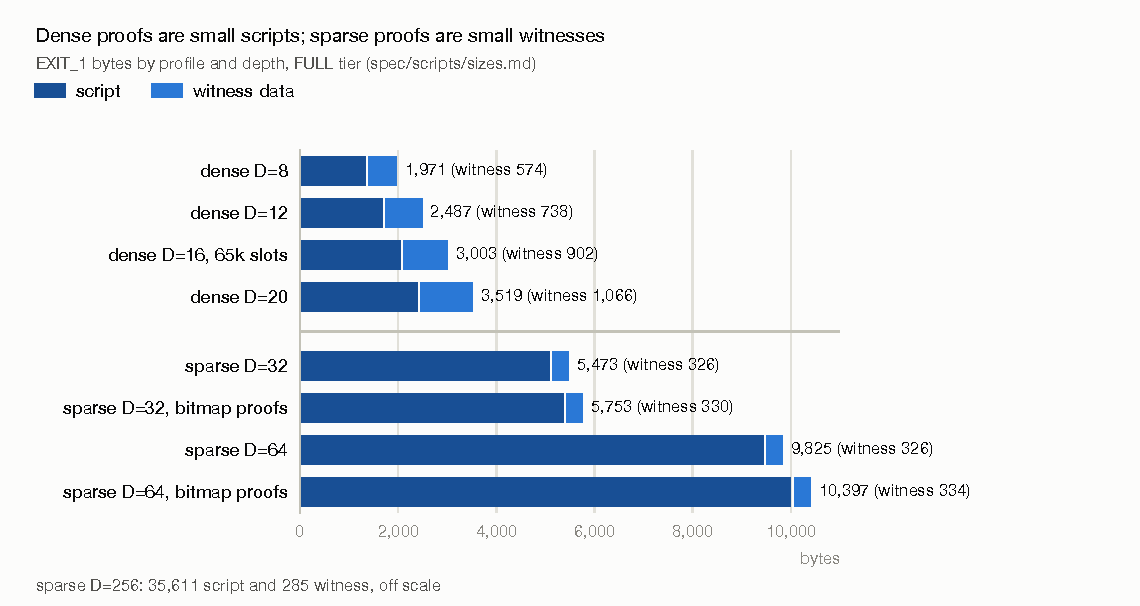
\includegraphics[width=\linewidth]{figures/exit-profiles.pdf}
\caption{\tr{EXIT}$_1$ bytes by profile and depth, FULL tier: dense
proofs are small scripts, sparse proofs small witnesses. Sparse rows are
measured on the six-leaf tree.}
\label{fig:cmp-profiles}
\end{figure}

Dense is therefore the default (spec~5.4, \path{spec/layertree.md}):
1.7 to 2.8 times cheaper per exit at $2^{16}$ members, with cohort grafts
at one price, sweeps at about $160\vB$ per leaf and every batch shape, at
the price of an operator who keeps the slot map. The sparse profile is kept,
specified and tested as the measured alternative, and for deployments that
are key-addressed registries.


% Short version only: the hypothetical native Merkle-sum opcode in full.
% The full version carries the same account in the evaluation section
% (body-eval.tex). Source: design/native-opcodes.md, tools/layertree_msu.py
% and tools/test_msu.py.

\subsection{A Native Merkle-Sum Opcode (Hypothetical)}\label{app:native}

Tapscript has no loops, so the tiers pay for every level of a path in
script, and that is the cost they change only by a constant. A hypothetical
\op{MERKLESUMUPDATE} would take a proof, an old node and a new node and
return the root of the old node's path and the root with the new node in
its place. The proof is a depth, a position and a bitmap naming the levels
that carry a sibling, then those 40-byte siblings; every other level uses
the empty node $\Emp_k$. The opcode adds the sums, fails on overflow past
$2^{64}$ or on a non-canonical proof, and costs $2\times$ the depth in
hashes, charged as BIP-440 varops. An old node equal to the new one is
plain verification. It replaces the unrolled fold and its arithmetic, so
with \op{CHECKCONTRACTVERIFY} binding the root and \op{TX} the payout, the
covenant compares byte strings only: no numeric operands, no padding and
no $2^{31}$ cap. Nobody has proposed it and nothing here depends on it; it
runs only in the simulator, behind a flag, in no tier and in no golden
script.

\tr{EXIT}$_1$ then has 252 bytes of script at every depth (2{,}101 in FULL
and 1{,}716 in CCV at $D = 16$) and one 40-byte witness sibling per
occupied level. Empty levels cost nothing, so a hashed-position tree
(Appendix~\ref{app:sparse}) costs no more than a dense one. For $2^k$
members in a key-addressed depth-64 tree the exit is about $381 + 10k\vB$
(541 at $2^{16}$, 701 at $2^{32}$), against $504 + 32.25k$ for FULL (1{,}020;
1{,}536) and $150k + 111$ for a transaction tree (2{,}511; 4{,}911):
$10\vB$ per doubling and no fixed depth. The $388\vB$ of
Figure~\ref{fig:cmp-anatomy} and the $520\vB$ of a full depth-16 tree are the
simulator's smaller model; 541 is the key-addressed one. The
\tr{CLAIM}$^{hm}$ redemption of a pending leaf is $626\vB$ at $2^{16}$
members against $1{,}136\vB$ in FULL.

It does little for batches. A rewrite or sweep is dominated by a
per-position step of about 376 bytes of script at $h = 6$, which the opcode
does not touch: settling pending receives costs $547\vB$ a pair at 64
positions (two transactions of $8{,}347$ and $9{,}155\vB$ at $2^{16}$
members, 24{,}065 bytes of script each against 25{,}036 in FULL). A
multi-leaf exit or a sweep would need several proofs in one call, or a way
to build a subtree root, which the proof format above does not express.
The price is that the opcode fixes in consensus this tree's node encoding,
empty-node chain, parent hash and overflow rule, so a different tree or a
format change would need a different opcode. That is why the work composes
proposed opcodes and proposes none, and treats the opcode as a measurement
of what the general approach pays, not as a tier.


\subsection{Where LayerTree Loses}\label{app:cmp-loses}

A member who never leaves alone pays almost nothing: about $3\vB$ for a
share of a graft, and about $160\vB$ in all if it leaves with its
cohort. A member
who does leave alone pays $1{,}020\vB$, about nine times a bare spend and
about twice a Lightning force close; the proof is the price of the shared
output. An on-chain update is $1{,}030\vB$, so payments must be off-chain
or batched. Renewing a lease costs $2{,}616\vB$ alone or $151\vB$ a
member in a signed cohort rewrite. Everything serialises through one
output, at about 25 single exits a block even when they cooperate,
which bounds how many
time-sensitive leaves one tree should host; fee pinning on that output is
outside the model. The sparse profile costs 1.7 to 2.8 times the dense
one and cannot graft or sweep. The MID tier caps a tree at $2^{31}$
satoshis. And the opcodes do not exist: every tier needs proposals that
are not active, three of them in a tapleaf version their proposals do
not define (Table~\ref{tab:assume}).

\subsection{How the Numbers Are Made}\label{app:cmp-model}

Every figure is a whole transaction on one model, the same in spec~11,
\path{spec/fee-analysis.md}, the evaluation of \S\ref{sec:eval} and
here: the measured script and witness and a 129-byte control block (the
eight-leaf reference taptree), plus a $946\WU$ skeleton (the tree input,
a P2WPKH fee input, the tree output, one P2TR payout and a P2WPKH change
output) and $172\WU$ per further payout, with
$\mathrm{vB} = \lceil \mathrm{WU}/4 \rceil$ once per transaction. A
transition without a payout (\tr{JOIN}, \tr{UPDATE}, \tr{CLAIM},
\tr{SPLIT}, a rewrite that only updates) is priced on $774\WU$, and the
fee-from-payout exit on $550\WU$. The model leaves out the witness item
count and the per-item length prefixes; \path{tools/measure_weight.py}
serialises the transactions the suites build and measures them
(\path{spec/scripts/weights.md}): $10.5\vB$ on a FULL \tr{EXIT}$_1$ at
$D = 16$, 10 in CCV, and 42.5 and 44.75 in MID and MIN, whose witnesses
carry each sibling as several small elements. The sizes come from
\path{tools/gen_listings.py} (\path{spec/scripts/sizes.md}), the fee
tables from \path{tools/fee_analysis.py}, and the figures of this
appendix from \path{tools/gen_cost_figures.py}; the baselines are models,
not measurements. The suites behind the sizes run 1{,}610 FULL, 1{,}391 MID,
57 MIN, 4{,}295 CCV and 220 channel-leaf checks, and 133 for the
hypothetical opcode, which stays out of every tier.
